\subsection{Idea}
Pre náš projekt potrebujeme vytvoriť tri veci. Potrebujeme aplikáciu, ktorá bude password managerom pre používateľa. Bude podporovať štandardné operácie už existujúcich password managerov, ako: pridanie hesla, vymazanie hesla, zobrazenie všetkých hesiel, kategorizácia hesiel. Aplikáciu obohatíme o novú funkcionalitu, ktorá nejakým spôsobom dostane heslá na cudzie zariadenie. A to všetko bezpečne.

Potrebujeme webstránku. Toto bude jediný komponent, ktorý bude prístupný na cudzom zariadení, keďže verejná webstránka je prístupná všade, kde existuje pripojenie k internetu. Na nej by sa používateľ verifikoval jednorázovým kódom alebo QR kódom a dostal by sa ku svojim dátam jednorázovo. Zo stránky by si údaje mohol skopírovať a používať počas používania cudzieho zariadenia.

Potrebujeme server. Kvôli rozsahu bakalárskej práce nebude podporovať synchronizáciu hesiel medzi zariadeniami používateľa. Teda, heslá budú existovať iba lokálne, vo filesystéme daného zariadenia. Server bude mať inú úlohu. Bude kľúčovým elementom, ktorý je zodpovedný za bránu von z ekosystému. Bez servera by nebolo možné dostať dáta z aplikácie von. Môžeme ho vnímať ako spojku medzi aplikáciou a webstránkou. Mal by nejakým spôsobom uchovávať dáta vyslané používateľom na obmedzenú dobu. 

Heslá uložené v zariadení, ktoré má nainštalovanú aplikáciu musia byť chránené. Preto v čase, keď je aplikácia vypnutá, musia byť heslá zašifrované. Kľúč od šifry musí byť kvalitným spôsobom ochránený a nedostupný. Cestovanie dát po sieti (od aplikácie na server, od servera na webstránku) musí prebiehať rovnako bezpečne. Ak nevieme toto docieliť, neposkytli sme riešenie na celú problematiku. Implementácia tohto problému musí na prvom mieste spĺňať podmienky silnej bezpečnosti moderného systému.

Zobrazme si tento návrh vizuálne pomocou jednoduchého diagramu na \figurename{ \ref{idea}}. Na základe tejto myšlienky budeme vyvíjať jednotlivé súčasti celého riešenia.

\begin{figure}[H]
  \centering
  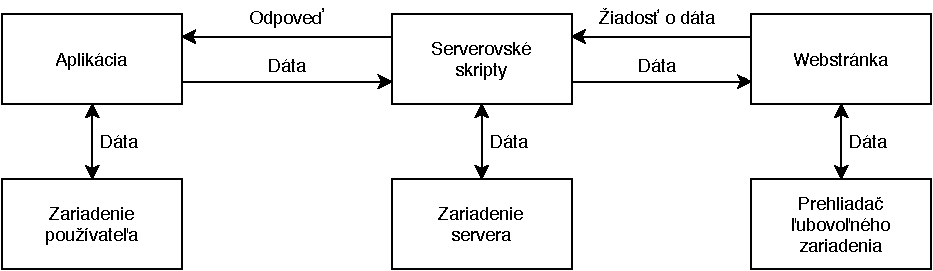
\includegraphics[width=15cm]{img/idea.pdf}
  \caption{Diagram implementácie nášho riešenia.}
  \label{idea}
\end{figure}

